% ltex: language=it
\chapter{Fondamenti}\label{chap:fondamenti} % (fold)
%
\section{Dati e Pattern}\label{sub:dati_e_pattern} % (fold)
I dati sono un ingrediente fondamentale del machine learning dove il comportamento dei modelli non è pre-programmato ma appreso dai dati stessi; termini come Data Science, Data Mining, Big Data enfatizzano il ruolo dei dati.
Generalmente un campione (multidimensionale) nel dominio di interesse è definito \textbf{Data-point}.
Si utilizza \textbf{Pattern} come sinonimo di data-point.
\\
Il \textbf{Pattern Recognition} è la disciplina che studia il riconoscimento dei pattern (non solo con tecniche di learning ma anche con algoritmi pre-programmati).
L'intersezione con il Machine Learning è molto ampia.
\subsection{Tipi di Pattern}\label{sec:tipi_di_pattern} % (fold)
\paragraph{Numerici}\label{par:numerici} % (fold)
Sono valori associati a caratteristiche misurabili o conteggi.
Tipicamente continui in ogni caso soggetti a ordinamento.
Rappresentabili naturalmente come vettori numerici nello spazio multidimensionale.
L'estrazione di caratteristiche da segnali (come immagini o suoni) produce vettori numerici detti anche feature vectors.
% paragraph Numerici (end)
\paragraph{Categorici}\label{par:categorici} % (fold)
Sono valori associati a caratteristiche qualitative e alla presenza/assenza di una caratteristica, talvolta ordinati.
Naturalmente gestiti da sistemi a regole e alberi di classificazione.
Attraverso tecniche di \textit{encoding}, o \textit{embedding}, è possibile mapparli su numeri, e quindi utilizzare modelli che operano solo su dati numerici.
Attenzione a \textit{ordinal encoding} arbitrari che non preservano semantica.
% paragraph Categorici (end)
% subsection Tipi di Pattern (end)
\paragraph{Sequenze}\label{par:sequenze} % (fold)
Pattern sequenziali con relazioni spaziali o temporali, spesso di lunghezza variabile.
La posizione nella sequenza e le relazioni con i predecessori e successori sono molto importanti.
\\
Allineamento spaziale/temporale, e <<memoria>> per tener conto del passato.
\\
Approcci moderni: Deep-learning: Long Short-Term Memory (LSTM), Transformers.
% paragraph Sequenze (end)
\paragraph{Altri dati strutturati}\label{par:altri_dati_strutturati} % (fold)
Output organizzati in strutture complesse quali alberi e grafi.
Applicazioni in Bioinformatics, Natural Language Processing, Speech Recognition, ecc.
Esempio nella traduzione di una frase in linguaggio naturale, l'output desiderato è l'insieme dei \textit{parse tree} plausibili.
% paragraph Altri dati strutturati (end)
\paragraph{Dati Tabulari}\label{par:dati_tabulari} % (fold)
In molte applicazioni aziendali, i dati sono organizzati in una tabella, come nel modello relazionale dei DBMS, nelle cui colonne troviamo gli attributi (features) e nelle righe i record (data point).
Le colonne possono avere un formato numerico o categorico, e sono eterogenee.
I dati possono essere incompleti e fortemente sbilanciati; non è semplice definire una metrica di similarità tra record.
\\
Le tecniche di deep learning hanno superato i metodi pre-esistenti nelle applicazioni che lavorano con dati omogenei non strutturati (immagini, audio, linguaggio), ma non sono altrettanto competitive su dati tabulari.
% paragraph Dati Tabulari (end)
\paragraph{Encoding}\label{par:encoding} % (fold)
Dato un campo materiale con i seguenti $5$ valori possibili: $\{$Acciaio, Cemento, Ghisa, Polietilene, PVC$\}$ è possibile codificarlo in due modi:
\begin{definition}{One-Hot Encoding}{}
    Si rimuove il campo e al suo posto si aggiungono tanti campi (o colonne) quanti sono i valori distinti ($5$ in questo caso).
    Ciascun campo è associato a un materiale diverso e può assumere sono valore $0/1$, dove $1$ indica che il pattern è di quel materiale.
    \\
    Svantaggioso con un numero elevato di pattern possibili.
\end{definition}
\begin{definition}{Ordinal Encoding}{}
    Si trasforma il campo originale in campo numerico associando ai materiali dei valori ordinali.
    \\
    Alcuni modelli interpretano numeri vicini come fattore di somiglianza.
\end{definition}
Fortunatamente i multi-classificatori basati su alberi tollerano bene l'ordinal encoding e spesso non è necessario ricorrere a one-hot encoding o altri embedding più complessi.
% paragraph Encoding (end)
%
\subsection{Classificazione}\label{sub:classificazione} % (fold)
\begin{definition}{Classificazione}{clsf}
    Operazione di assegnazione di una \textbf{classe} a un pattern, si usa spesso anche il termine riconoscimento.
    È necessario apprendere una funzione capace di eseguire il mapping dallo spazio dei pattern allo spazio delle classi.
    Nel caso di due sole classi si usa il termine \textit{binary classification}, con più di due classi \textit{multi-class classification}.
\end{definition}
\begin{definition}{Classe}{}
    Una classe è un insieme di pattern aventi proprietà comuni. Il concetto di classe è semantico e dipende strettamente dall'applicazione.
\end{definition}
\begin{example}{Problemi di Classificazione}{}
    \begin{itemize}
        \item Spam detection;
        \item Credit Card fraud detection;
        \item Face recognition;
        \item Pedestrian recognition;
        \item Medical diagnosys;
        \item Stock Trading;
    \end{itemize}
\end{example}
%
% subsection Classificazione (end)
%
\subsection{Regressione}\label{sec:regressione} % (fold)
\begin{definition}{Regressione}{}
    Assegnazione di un valore continuo a un pattern, utile per la predizione di valori continui.
    \\
    Risolvere un problema di regressione corrisponde ad apprendere una funzione approssimante delle coppie <<input/output>> date.
\end{definition}
\begin{cimage}
    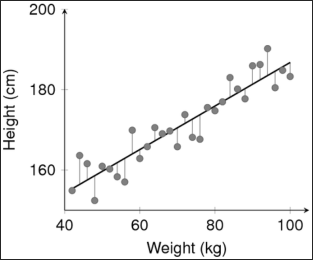
\includegraphics[width=.45\textwidth]{assets/weight-height-estimation.png}
    \caption{Stima dell'altezza di una persona in base al peso}\label{fig:weight-height-estimation}
\end{cimage}
\begin{example}{Problemi di Regressione}{}
    \begin{itemize}
        \item Stima di prezzi di vendita di appartamenti nel mercato immobiliare;
        \item Stima del rischio per compagnie assicurative;
        \item Predizione energia prodotta da impianto fotovoltaico;
        \item Modelli sanitari di predizione dei costi;
        \item Object detection;
    \end{itemize}
\end{example}
% subsection Regressione (end)
%
\subsection{Clustering}\label{sec:clustering} % (fold)
\begin{definition}{Clustering}{}
    Individuare gruppi (cluster) di pattern con caratteristiche simili.
    Le classi del problema non sono note e i pattern non etichettati: la natura non supervisionata del problema lo rende più complesso della classificazione.
    Spesso il numero dei cluster è noto a priori, ognuno dei quali se individuati nell'apprendimento possono essere poi utilizzati come classi.
\end{definition}
\begin{cimage}
    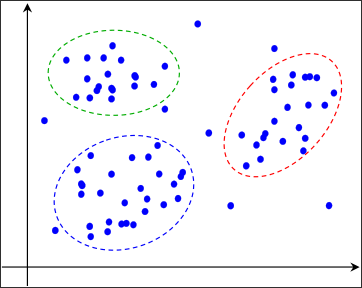
\includegraphics[width=.45\textwidth]{assets/clusters.png}\label{fig:clusters}
\end{cimage}
\begin{example}{Problemi di Clustering}{}
    \begin{itemize}
        \item Marketing: definizione di gruppi utenti in base ai consumi;
        \item Genetica: raggruppamento di individui sulla base di analogie del DNA;
        \item Bioinformatica: partizionamento dei geni in gruppi con caratteristiche simili;
        \item Visione: segmentazione non supervisionata.
    \end{itemize}
\end{example}
% subsection Clustering (end)
%
\subsection{Riduzione Dimensionalità}\label{sec:riduzione_dimensionalita} % (fold)
\begin{definition}{Riduzione di dimensionalità}{}
    Ridurre il numero di dimensioni dei pattern di input.
    Consiste nell'apprendimento di un mapping da $\R^d$ a $\R^k$, con $k < d$.
    L'operazione comporta una perdita di informazioni, l'obiettivo principale è quello di conservare le informazioni <<importanti>>.
    La definizione formale di importanza dipende dall'applicazione.
\end{definition}
Molto utile per rendere trattabili problemi con dimensionalità molto elevata, per scartare informazioni ridondanti e/o instabili, e per visualizzare in 2D o 3D pattern con $d > 3$.
\begin{cimage}
    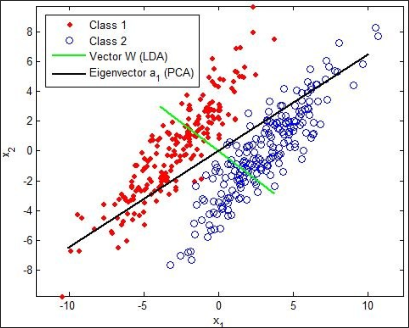
\includegraphics[width=.5\textwidth]{assets/rid-dim-es.png}
\end{cimage}
% subsection Riduzione Dimensionalita (end)
% section Dati e Pattern (end)
%
\section{Representation Learning}\label{sec:representation_learning} % (fold)
Il successo di molte applicazioni di machine learning dipende dall'efficacia di rappresentazione dei pattern in termini di features.
La definizione di features ad-hoc (\textbf{hand-crafted}) per le diverse applicazioni prende il nome di \textit{feature engineering}.
\\
Gran parte delle tecniche di deep learning, come le \textit{convolutional neural networks}, apprendono le feature direttamente dai raw data.
Utilizzano come input i raw data ed estraendo automaticamente da essi le feature necessarie per risolvere il problema di interesse.
\paragraph{Problemi nel dominio Visione}\label{par:problemi_nel_dominio_visione} % (fold)
\begin{itemize}
    \item \textbf{Classification}: determina la classe di un oggetto;
    \item \textbf{Localization}: determina la classe dell'oggetto e la sua posizione nell'immagine;
    \item \textbf{Detection}: per ogni oggetto presente determina la classe e la posizione nell'immagine;
    \item \textbf{Segmentation}: al posto di una bounding box, etichetta i singoli pixel dell'immagine in classi con indici delle classi.
        Applicazioni in ambito telerilevamento, immagini mediche, guida automatica.
\end{itemize}
% paragraph Problemi nel dominio Visione (end)
%
% section Representation Learning (end)
%
\section{Modelli Discriminativi vs Generativi}\label{sec:modelli_discriminativi_vs_generativi} % (fold)
I modelli \textbf{discriminativi} (classificatori), hanno l'obiettivo di assegnare un nuovo datapoint a una classe.
La cosa importante è apprendere il decision boundary che separa le classi.
\begin{cimage}
    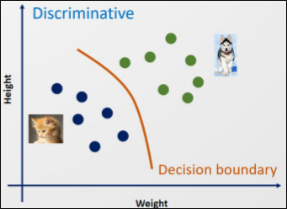
\includegraphics[width=.6\textwidth]{assets/mod-discri.png}
    \caption{Classificazione $\equiv$ su quale lato del decision boundary cade il nuovo dato?}
\end{cimage}
I modelli \textbf{generativi} apprendono (esplicitamente/implicitamente) la distribuzione probabilistica degli esempi usati per il loro addestramento.
Dopo l'addestramento possono:
\begin{itemize}
    \item generare nuovi dati sintetici a partire da numeri casuali;
    \item modificare o trasformare l'input fornito;
    \item classificare l'input comparando le probabilità che sia generato dalle diverse classi;
\end{itemize}
\begin{cimage}
    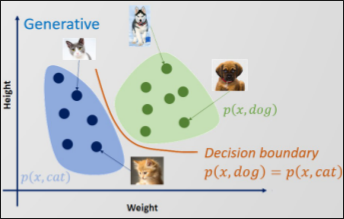
\includegraphics[width=.6\textwidth]{assets/mod-gen.png}
\end{cimage}
% section Modelli Discriminativi vs Generativi (end)
\section{Generative AI}\label{sec:generative_ai} % (fold)
La moderna \ac{genai} fa largo uso di modelli generativi basati su reti neurali profonde (GAN, VAE, LLM).
\begin{warning}
    Il termine generative può essere ambiguo in quanto le tecniche di \ac{genai} possono anche risolvere problemi che non richiedono la produzione creativa di contenuti.
    Pertanto generativo, da non confondere con creativo, si riferisce ai sottostanti modelli generativi usati.
\end{warning}
\begin{cimage}
    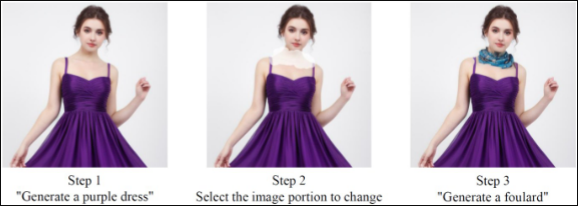
\includegraphics[width=.6\textwidth]{assets/gen-es.png}
\end{cimage}
% section Generative AI (end)
%
\section{Apprendimento}\label{sec:apprendimento} % (fold)
\begin{definition}{Addestramento Supervisionato}{}
    Sono note le classi dei pattern utilizzati per l'addestramento:
    \begin{itemize}
        \item il training set è etichettato;
        \item situazione tipica nella classificazione, regressione e in alcune tecniche di riduzione di dimensionalità;
    \end{itemize}
\end{definition}
\begin{definition}{Addestramento Non Supervisionato}{}
    Non sono note le classi dei pattern utilizzati per l'addestramento.
    \begin{itemize}
        \item il training set non è etichettato;
        \item situazione tipica nel clustering e nella maggior parte di tecniche di riduzione di dimensionalità;
        \item anomaly detection è spesso considerata un'applicazione unsupervised: si hanno molti esempi di funzionamento normale, ma pochi casi di errore;
    \end{itemize}
\end{definition}
\begin{definition}{Addestramento Semi-Supervisionato}{}
    \begin{itemize}
        \item il training set è etichettato parzialmente;
        \item la distribuzione dei pattern non etichettati può aiutare a ottimizzare la regola di classificazione;
    \end{itemize}
\end{definition}
\begin{definition}{Batch}{}
    L'addestramento è effettuato una sola volta su un training set dato.
    Una volta terminato il training, il sistema passa in <<working mode>> e non è in grado di apprendere ulteriormente.
    Attualmente la maggior parte dei sistemi di machine learning opera in questo modo.
\end{definition}
\begin{definition}{Incrementale}{}
    A seguito dell'addestramento iniziale, sono possibili ulteriori sessioni di addestramento:
    \begin{itemize}
        \item \textbf{scenari}: sequenze di Batch, Unsupervised Tuning;
        \item \textbf{rischio}: Catastrofic Forgetting (il sistema dimentica quello che ha appreso in precedenza);
    \end{itemize}
\end{definition}
\begin{definition}{Naturale}{}
    Addestramento continuo (per tutta la vita): attivo in working mode, coesistenza di approccio supervisionato e non.
\end{definition}
%
% section Apprendimento (end)
%
\section{Reinforcement Learning (RL)}\label{sec:reinforcement_learning_rl_} % (fold)
L'obiettivo è apprendere un comportamento ottimale a partire dalle esperienze passate.
Un agente esegue azioni che modificano l'ambiente, provocando messaggi da uno stato all'altro.
Quando l'agente ottiene risultati positivi riceve una ricompensa (\textit{reward}) che però può essere temporalmente ritardata rispetto all'azione, o alla sequenza di azioni, che l'hanno determinata.
L'obiettivo è quello di apprendere l'azione ottimale in ciascun stato, in modo da massimizzare la somma dei reward ottenuti nel lungo periodo.
\begin{cimage}
    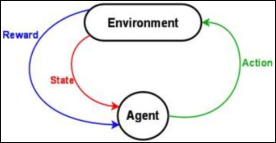
\includegraphics[width=.6\textwidth]{assets/rl.png}
\end{cimage}
Nella pratica è molto difficile ottenere esempi che siano allo stesso tempo corretti e rappresentativi di tutte le situazioni in cui l'agente deve agire.
Pertanto il classico approccio supervisionato non è facilmente applicabile.
Numerose sono le applicazioni in robotica, e uno degli approcci più noti è il \textbf{Q Learning}.
\\
Una sua estensione (deep) denominata \ac{deeprl} è alla base dei successi ottenuti da Google DeepMind.
% section Reinforcement Learning (RL) (end)
%
\section{Parametri e Funzione Obiettivo}\label{sec:parametri_e_funzione_obiettivo} % (fold)
In generale, il comportamento di un modello $M$ di machine learning è regolato da un set di parametri $\te$.
Per rendere esplicita questa dipendenza indichiamo il modello come $M\pt \te$.
L'apprendimento consiste nel determinare il valore ottimo $\te[*]$ di questi parametri.
\\
Dato un training set $Train$ e un insieme di parametri, la \textbf{funzione obiettivo} $f\pt{Train, M\pt \te}$ può indicare:
\begin{itemize}
    \item l'ottimalità della soluzione (da massimizzare) \[ \te[*] = \argmax_{\te}{f\pt{Train, M\pt \te}} \]
    \item oppure l'errore o perdita (\textbf{loss-function}) da minimizzare \[ \te[*] = \argmin_{\te}{f\pt{Train, M\pt \te}} \]
\end{itemize}
$f\pt{Train, M\pt \te}$ può essere ottimizzata:
\begin{itemize}
    \item \textbf{esplicitamente}, con metodi che operano a partire dalla sua definizione matematica;
    \item \textbf{implicitamente}, utilizzando euristici che modificano i parametri in modo coerente con $f$;
\end{itemize}
% section Parametri e Funzione Obiettivo (end)
%
\subsection{Iperparametri}\label{sec:iperparametri} % (fold)
Stabilito il modello da utilizzare, prima dell'apprendimento vero e proprio, deve essere definito il valore dei cosiddetti \textbf{iperparametri}.
\begin{definition}{Iperparametri}{iperparam}
    Gli iperparametri $H$ definiscono i dettagli architetturali del modello e della corrispondente procedura di training.
    Per rendere esplicita anche questa dipendenza si utilizza $M\pt{H, \te}$.
\end{definition}
\begin{example}{}{}
    \begin{itemize}
        \item numero di neuroni in una rete neurale;
        \item numero di vicini $k$ in un classificatore $k$-NN;
        \item grado di un polinomio utilizzato in una regressione;
        \item tipo di loss function;
    \end{itemize}
\end{example}
\\
Per l'addestramento si procede con un approccio a due livelli: a livello esterno si fissano gli iperparametri $H$; a livello interno si esegue l'apprendimento e si valutano le prestazioni.
Al termine della procedura si scelgono gli iperparametri $H^*$ che hanno fornito prestazioni migliori.
\begin{cimage}
    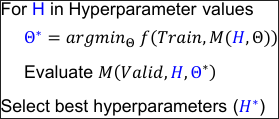
\includegraphics[width=.4\textwidth]{assets/sel-iperpar.png}
\end{cimage}
% subsection Iperparametri (end)
\subsection{Training, Validation, Test}\label{sec:training_validation_test} % (fold)
\begin{definition}{Training Set}{ts}
    Il Training Set è l'insieme di pattern su cui addestrare il modello, trovando il valore ottimo per i parametri $\te$.
\end{definition}
\begin{definition}{Validation Set}{}
    Il Validation Set è l'insieme di pattern su cui tarare gli iperparametri $H$ (ciclo esterno).
\end{definition}
\begin{definition}{Test Set}{}
    Il Test Set è l'insieme di pattern su cui valutare le prestazioni finali.
\end{definition}
\\
Nei benchmark classici di machine learning la suddivisione dei pattern in Train, Valid e Test è spesso predefinita, per rendere confrontabili i risultati.
In caso contrario è compito del progettista definire la suddivisione.
Si può optare per:
\begin{itemize}
    \item Set disgiunti;
    \item K-fold Cross-Validation;
\end{itemize}
%
\paragraph{Set Disgiunti}\label{par:set_disgiunti} % (fold)
Se i dati sono sufficientemente numerosi per la complessità del problema e del modello scelto, si possono usare i Set Disgiunti.
Aumentare la partizione di Train consente di addestrare meglio il modello.
D'altro canto Validation e Test troppo piccoli non permettono di misurare con sufficiente confidenza le prestazioni e la generalizzazione.
\\
La dimensione del validation/test dipende anche dall'entità dell'errore atteso.
Se l'errore di classificazione del sistema è del $10\%$, con un test set di $2500$ esempi avremo $250$ casi di errore.
Se l'errore è lo $0.2\%$ avremo solo $5$ errori con conseguente scarsa affidabilità statistica.
\emptyln{}
Lo split può essere random (shuffling) oppure mirato, es. per mantenere separati periodi temporali di train e set.
Nel caso di \textit{serie temporali}, dove il sistema è addestrato su un periodo storico e produrre previsioni per un periodo successivo, uno split random non è corretto (porta a una sovrastima delle prestazioni) in quanto il training set include data point temporalmente vicini a quelli di test.
% paragraph Set Disgiunti (end)
%
\paragraph{K-fold Cross-Validation}\label{par:paragraph_name} % (fold)
Una scelta più robusta degli iperparametri si ottiene con la procedura di K-fold Cross-Validation.
Nell'ipotesi di $15000$ pattern totali e $k = 5$:
\begin{itemize}
    \item $5000$ pattern sono scorporati a priori per il Test;
    \item i $10000$ pattern rimanenti sono suddivisi in $5$ gruppi (fold) da $2000$ pattern ciascuno;
\end{itemize}
\begin{cimage}
    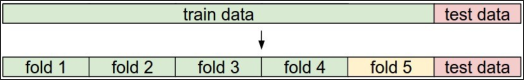
\includegraphics[width=.8\textwidth]{assets/k-fold-cross-val.png}
\end{cimage}
Per ogni combinazione di iperparametri $H_i$ che si vuole valutare:
\begin{itemize}
    \item si esegue $5$ volte il training scegliendo uno dei fold come Valid e i $4$ rimanenti come Train;
    \item si calcola l'accuratezza $avg\_acc_i$ come media/mediana delle $5$ accuratezze sui rispettivi Valid;
\end{itemize}
Si sceglie la combinazione di iperparametri con migliore $avg\_acc$.
Scelti gli iperparametri ottimali si riaddestra il modello su tutto il training set ($5$ fold) e, solo a questo punto, si verificano le prestazioni sul \textit{test set}.
\begin{note}[Leave-one-out]{}
    Caso estremo di cross-validation dove i fold hanno dimensione $1$.
    Visto il costo computazionale, si utilizza quando i pattern sono pochi.
\end{note}
% paragraph K-fold Cross-Validation (end)
%
\paragraph{Cherry Picking}\label{par:cherry_picking} % (fold)
Uno studio recente ha condotto una revisione sistematica di $27$ lavori scientifici che utilizzano il machine learning per il trading di azioni.
Tutti i lavori considerati dichiarano predizioni accurate e strategie profittevoli.
Al tempo stesso non si ha evidenza di casi reali di chiaro successo in ambito AI-driven trading.
\\
La quasi totalità dei lavori considerati esegue molteplici esperimenti per la scelta della strategia/modello migliore.
I modelli sono poi validati sul test set, e viene scelto il migliore (\textbf{cherry picking}).
In questo modo si ha \textit{overfitting} del test set.
\begin{warning}
    Non usare il test set per orientare le scelte durante lo sviluppo di un sistema, specialmente quando le dimensioni del test set sono limitate ed è forte il rischio di overfitting.
\end{warning}
% paragraph Cherry Picking (end)
% subsection Training, Validation, Test (end)
%
\subsection{Partizionare i Dati}\label{sec:partizionare_i_dati} % (fold)
Partizionare i dati in dati in Training, Validation e Test, richiede in genere di generare gli indici degli elementi da assegnare ai diversi insieme per poi procedere alla suddivisione facendo attenzione a dividere nello stesso modo anche le etichette o valori target.
\\
La funzione \texttt{train\_test\_split} di Scikit Learn automatizza questa fase, a partire dalle proporzioni specifiche in input, fornendo anche supporto per shuffling (ordinamento casuale dei pattern) e stratification.
\\
Relativamente a Cross Validation Scikit Learn mette a disposizione la funzione \texttt{cross\_val\_score} che a partire da un unico training set e il numero $K$ di fold, valuta $K$ volte il sistema e ritorna un array di $K$ score.
% subsection Partizionare i Dati (end)
%
\subsection{Selezione Automatica Iperparametri}\label{sec:selezione_automatica_iperparametri} % (fold)
La ricerca di valori ottimali per gli iperparametri può essere lunga e noiosa.
\paragraph{Grid Search}\label{par:grid_search} % (fold)
Per ogni iperparametro si definisce un insieme di valori da provare.
Il sistema è valutato su tutte le combinazioni di valori di tutti gli iperparametri.
Può essere molto costoso: raffinamento incrementale dei valori.
Prestare particolare attenzione se vengono selezionato valori di bordo per uno o più iperparametri.
\begin{example}{Esempio con funzione \texttt{GridSearchCV}}{}
    Come mostrato in \cref{fig:grid-search-es}, ogni $\{\}$ corrisponde a una grid search:
    \begin{itemize}
        \item nella prima si valuta un classificatore SVM con kernel lineare e con $4$ valori di $C \to 4$ valutazioni;
        \item nella seconda si valuta il classificatore con kernel RBF, $4$ valori di $C$ e $2$ valori di $\gm \to 8$ valutazioni;
        \item in totale $12$ valutazioni, ciascuna delle quali fatta con Cross Validatio;
    \end{itemize}
\end{example}
\begin{cimage}
    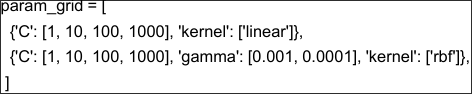
\includegraphics[width=.6\textwidth]{assets/grid-search-es.png}
    \caption{Esempio di iperparamentri}\label{fig:grid-search-es}
\end{cimage}
% paragraph Grid Search (end)
\paragraph{Random Search}\label{par:random_search} % (fold)
Sorteggia casualmente valori di iperparametri dai range/distribuzioni specificati/e, eseguendo un numero prefissato di iterazioni.
Funzione \texttt{RandomizedSearchCV}.
% paragraph Random Search (end)
% subsection Selezione Automatica Iperparametri (end)
%
\subsection{Auto-ML}\label{sec:auto_ml} % (fold)
I sistemi Auto-ML effettuano la scelta automatica del modello migliore (es. SVM, Random Forest, Rete Neurale MLP), per la risoluzione di un problema.
Oltre al modello possono essere scelte automaticamente tecniche di data/feature processing.
L'approccio naive prevede un ulteriore <<ciclo esterno>> è sul tipo di modello.
\begin{cimage}
    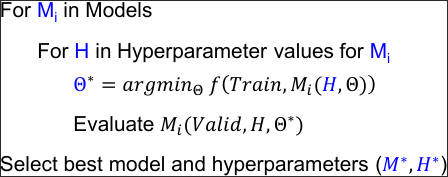
\includegraphics[width=.6\textwidth]{assets/mod-picker-automl.png}
\end{cimage}
Auto-ML è solitamente eseguito su risorse remote in Cloud (dimensionate opportunamente), ma esistono versioni per computazione locale, ad esempio Auto-Sklearn.
\begin{cimage}
    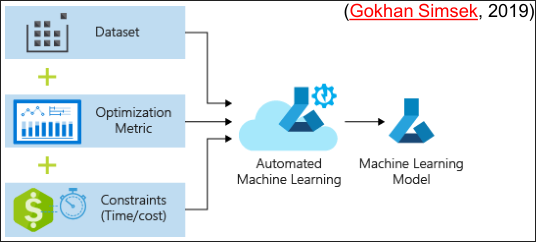
\includegraphics[width=.8\textwidth]{assets/automl.png}
\end{cimage}
% subsection Auto-ML (end)
%
\section{Metriche per la misura di prestazioni}\label{sub:metriche_per_la_misura_di_prestazioni} % (fold)
Una possibilità consiste nell'utilizzare direttamente la funzione obiettivo per quantificare le prestazioni.
In genere però si preferisce una misura legata direttamente alla semantica del problema.
In un problema di Classificazione \cref{sub:classificazione}, l'accuratezza di classificazione $\ps{0\dots100\%}$ è la percentuale di pattern correttamente classificati.
L'errore di classificazione è il complemento.
\[
    \begin{matrix}
        Accuratezza = \dfrac{\text{pattern correttamente classificati}}{\text{pattern classificati}} \\ \\
        Errore = 100\% - Accuratezza
    \end{matrix}
\]
Attenzione ai problemi di classificazione con cardinalità classi molto sbilanciate:
\begin{example}{}{}
    In un problema di classificazione binaria, se una delle due classi è rara, un classificatore <<dummy>> che non la predice mai potrebbe raggiungere un'accuratezza di classificazione vicina al $100\%$.
    Meglio usare Precision/Recall in questo caso.
\end{example}
Nei problemi di Regressione \cref{sec:regressione}, si valuta in genere l'\ac{rmse}, ovvero la radice media dei quadrati degli scostamenti tra valore vero e valore predetto.
\[
    RMSE = \sqrt{\dfrac{1}{N}\sum_{i = 1\dots N}{\pt{pred_i - true_i}^2}}
\]
%
\subsection{Matrice di Confusione}\label{sec:matrice_di_confusione} % (fold)
La matrice di confusione (confusion matrix) è molto utile nei problemi di classificazione \cref{sub:classificazione}, per capire come sono distribuiti gli errori.
Nell'esempio di un problema di classificazione digit ($10$ classi):
\begin{itemize}
    \item assumiamo che sulle righe ci siano le classi \texttt{True} (o \textit{Real} o \textit{Actual}), e sulle colonne le classi \texttt{Predicted} (non sempre così: a vole vengono scambiate);
    \item una cella $(r, c)$ riporta il numero di casi in cui il sistema ha predetto di classe $c$ un pattern di classe vera $r$;
    \item idealmente la matrice dovrebbe essere diagonale.
        Valori elevati (fuori diagonale) indicano casi di errore;
\end{itemize}
\begin{cimage}
    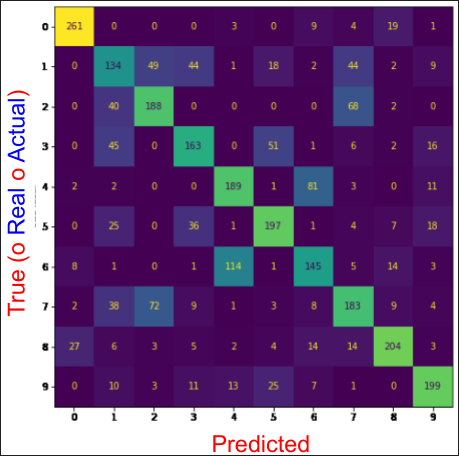
\includegraphics[width=.6\textwidth]{assets/conf-matrix.png}
\end{cimage}
La matrice può essere normalizzata per righe (classi \textit{True}) per passare da numero di errori a percentuali di errore.
Dopo la normalizzazione i valori sulle righe hanno somma $1$.
\begin{quote}{}{}
    Funzione \texttt{plot\_confusion\_matrix} disponibile in scikit-learn
\end{quote}
\begin{cimage}
    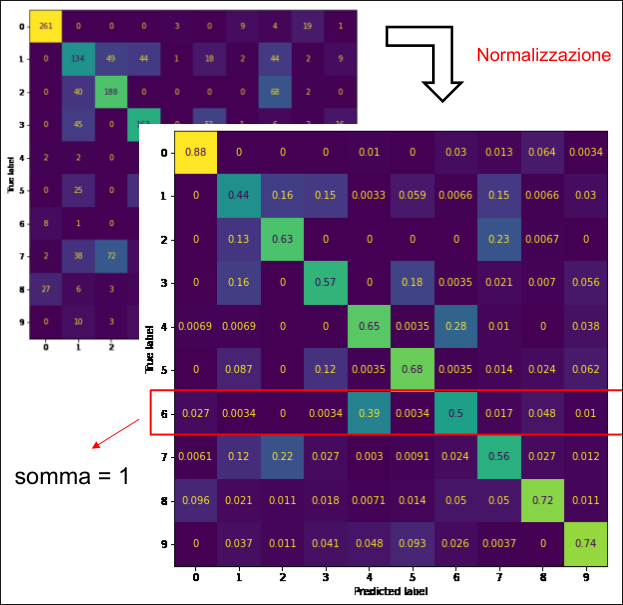
\includegraphics[width=.6\textwidth]{assets/norm-conf-matrix.png}
    \caption{Matrice di confusione normalizzata}\label{fig:norm-conf-matrix}
\end{cimage}
% subsection Matrice di Confusione (end)
%
\subsection{Classificazione Binaria}\label{sec:classificazione_binaria} % (fold)
Dato un \textbf{classificatore binario}, e $T = P + N$ pattern da classificare ($P$ positivi e $N$ negativi), il risultato di ciascuno dei tentativi di classificazione può essere:
\begin{itemize}
    \item \textbf{\ac{tp}}: un pattern positivo è stato correttamente assegnato ai positivi;
    \item \textbf{\ac{tn}}: un pattern negativo è stato correttamente assegnato ai negativi;
    \item \textbf{\ac{fp}}: un pattern \textit{negativo} è stato erroneamente assegnato ai positivi; detto anche errore di \textbf{Tipo I} o \textbf{False};
    \item \textbf{\ac{fn}}: un pattern \textit{positivo} è stato erroneamente assegnato ai negativi; detto anche errore di \textbf{Tipo II} o \textbf{Miss};
\end{itemize}
Passando da errori a frequenze/probabilità, che corrisponde a normalizzare per righe la \hyperref[sec:matrice_di_confusione]{Matrice di Confusione}:
\[
    \begin{matrix}
        \text{\acf{tpr}} = \dfrac{TP}{P} \\ \\
        \text{\acf{tnr}} = \dfrac{TN}{N} \\ \\
        \text{\acf{fpr}} = \dfrac{FP}{N} \\ \\
        \text{\acf{fnr}} = \dfrac{FN}{P} \\ \\
    \end{matrix}
\]
Con questa notazione l'accuratezza di classificazione può essere scritta come:
\[
    Accuracy = \dfrac{TP + TN}{T = P + N}
\]
\\
I $4$ casi (\ac{tn}, \ac{fp}, \ac{fn}, \ac{tp}) sono facilmente collocabili sulle $4$ celle della matrice di confusione ($2\times 2$).
Le relative frequenze (\ac{tnr}, \ac{fpr}, \ac{fnr}, \ac{tpr}) occupano le stesse posizioni sulla matrice di confusione normalizzata.
\begin{cimage}
    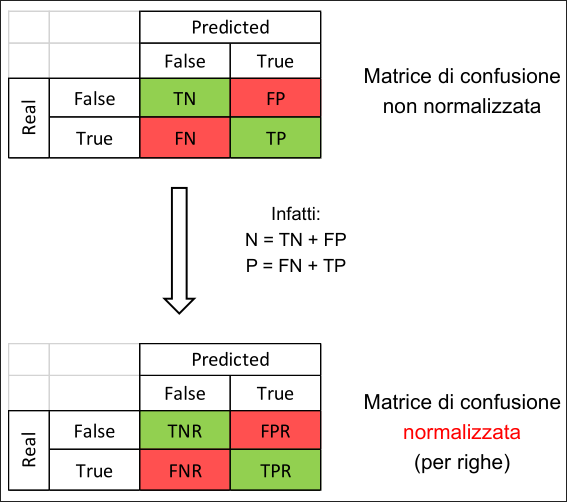
\includegraphics[width=.6\textwidth]{assets/conf-mat-err.png}
    \caption{Errori sulla matrice di confusione normalizzata e non}\label{fig:conf-mat-err}
\end{cimage}
%
% subsection Classificazione Binaria (end)
%
\subsection{\ac{det} e \ac{roc}}\label{sec:det_e_roc} % (fold)
L'output di un classificatore è spesso \textbf{probabilistico} (valore continuo in $0\dots1$).
In un problema di classificazione binaria i pattern possono essere predetti come positivi (o negativi) confrontando l'output (della classe positiva) con una soglia $t$.
Soglie restrittive (elevate) riducono i false positive a discapito dei false negative; viceversa soglie tolleranti (basse) riducono i false negative a discapito dei false positive.
\\
\begin{cimage}
    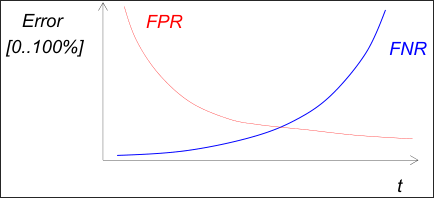
\includegraphics[width=.6\textwidth]{assets/fpr-fnr-error-t.png}
    \caption{False Positive e Negative Rate al variare della tolleranza}\label{fig:fpr-fnr-error-t}
\end{cimage}
Le due curve in \cref{fig:fpr-fnr-error-t}, possono essere <<condensate>> in una curva \ac{det} che nasconde la soglia.
\begin{cimage}
    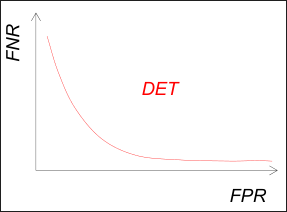
\includegraphics[width=.4\textwidth]{assets/det-curve.png}
\end{cimage}
Piuttosto usata è anche la rappresentazione \ac{roc} che in ordinata riporta True Positive invece di False Negative (ribaltata verticalmente rispetto a \ac{det}).
\begin{cimage}
    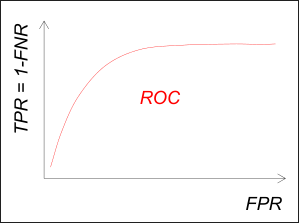
\includegraphics[width=.4\textwidth]{assets/roc-curve.png}
\end{cimage}
\paragraph{Area Under Curve (AUC)}\label{par:area_under_curve_auc_} % (fold)
Area Under Curve (AUC)Quale dei due sistemi (rosso, blu) è migliore dell'altro?
\begin{cimage}
    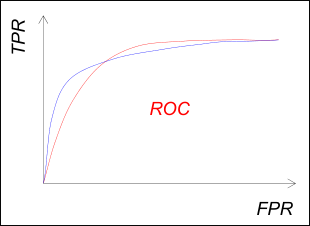
\includegraphics[width=.4\textwidth]{assets/sys-com-roc.png}
\end{cimage}
\begin{quote}
    Il sistema migliore è quello la cui curva è più <<alta>>, ma in questo caso le curve si intersecano\dots{} e l'ottimalità dipende dal punto di lavoro desiderato.
\end{quote}
Un confronto può essere fatto <<mediando>> sui diversi punti di lavoro del sistema.
L'\textbf{area sotto la curva} \ac{roc}, chiamata \textbf{\ac{auc}}, è uno scalare in $\ps{0, 1}$ che caratterizza la prestazione media (maggiore è, meglio è).
Può essere calcolata come integrale numerico attraverso il metodo dei trapezi.
\begin{cimage}
    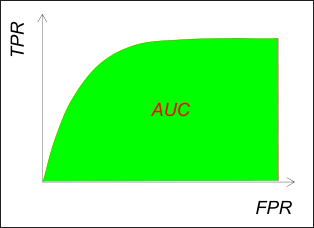
\includegraphics[width=.4\textwidth]{assets/auc.png}
\end{cimage}
%
% paragraph Area Under Curve (AUC) (end)
% subsection det e roc (end)
%
\subsection{Precision e Recall}\label{sec:precision_e_recall} % (fold)
Notazione molto usata in Information Retrieval e in generale nelle applicazioni di detection o di classificazione, con classi sbilanciate.
Precision/Recall sono definiti a partire da \ac{tn}, \ac{fp}, \ac{fn}, \ac{tp} (\hyperref[sec:classificazione_binaria]{classificazione binaria}).
\begin{itemize}
    \item \textbf{Precision}, indica quanto è accurato il sistema:
        \[
            Precision = \frac{TP}{TP + FP}
        \]
    \item \textbf{Recall}, indica quanto è selettivo (già disponibile nella matrice di confusione normalizzata):
        \[
            Recall = \frac{TP}{TP + FN} = \frac{TP}{P} = TPR
        \]
\end{itemize}
\begin{cimage}
    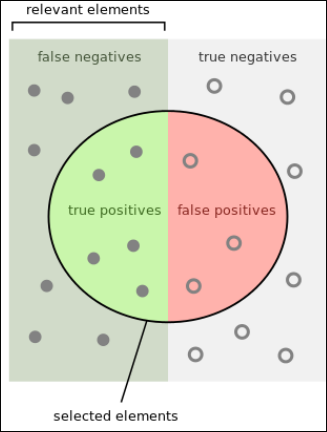
\includegraphics[width=.4\textwidth]{assets/prec-recall-cake.png}
    \caption{}\label{fig:prec-recall-cake}
\end{cimage}
\paragraph{Precision e Recall su matrice $2\times2$}\label{par:precision_e_recall_su_matrice_times_} % (fold)
La rappresentazione grafica più utile per comprendere Precision e Recall è la matrice di confusione $2\times2$ che evidenzia \ac{tn}, \ac{tp}, \ac{fp}, \ac{fn}:
\begin{cimage}
    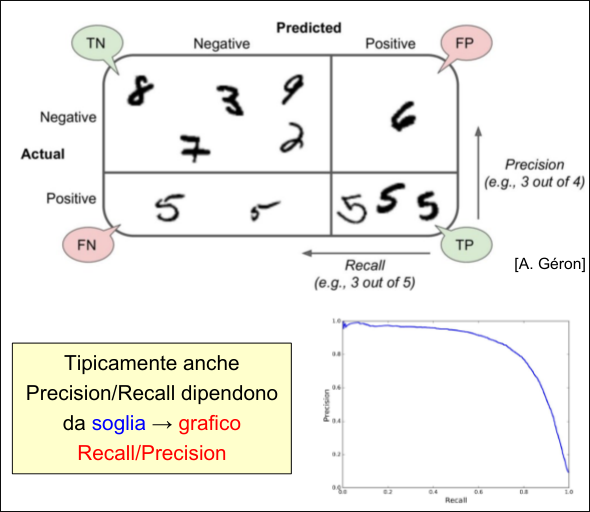
\includegraphics[width=.6\textwidth]{assets/prec-recall-2-2.png}
\end{cimage}
Nella classificazione multi-classe, precision e recall si possono calcolare per ciascuna classe (considerando la classe come Positive e gli esempi di tutte le altre come Negative), come nell'esempio sopra.
% paragraph Precision e Recall su matrice $2\times2$ (end)
% subsection Precision e Recall (end)
%
\subsection{Indicatori compatti}\label{sec:indicatori_compatti} % (fold)
Gli indicatori compatti (a singolo valore) sono utili per comparare l'accuratezza di diversi modelli.
\paragraph{F1-score}\label{par:f_score} % (fold)
Comprende valori continui in $0\dots1$, viene calcolato come \textit{media armonica} di Precision e Recall:
\[
    F1 - score = 2 \times \dfrac{Precision \times Recall}{Precision + Recall}
\]
La media armonica:
\begin{itemize}
    \item corrisponde alla media aritmetica se $Precision = Recall$;
    \item <<penalizza maggiormente>> rispetto alla media aritmetica quando i valori sono diversi;
\end{itemize}
% paragraph F1-score (end)
\paragraph{\acf{ap}}\label{par:_acf_ap_} % (fold)
È una sorta di \ac{auc} sul grafico Recall/Precision:
\[
    AP = \sum_n{\pt{R_n - R_{\dec n}}}P_n
\]
dove $P_n$ e $R_n$ sono i valori di precision e recall alla soglia $n$.
Differentemente da \ac{auc} si usa l'integrazione con rettangoli (e non trapezi) per evitare il risultato over-ottimistico.
\\
Nelle applicazioni dove è importante operare a Precision (o Recall) definiti meglio derivare esplicitamente dal grafico Recall/Precision:
\[
    \begin{matrix}
        Precision \text{ @ } Recall = X \\
        Recall \text{ @ } Precision = X
    \end{matrix}
\]
% paragraph \acf{ap} (end)
% subsection Indicatori compatti (end)
%
\subsection{Sensitivity e Specificity}\label{sec:sensitivity_e_specificity} % (fold)
In diagnostica medica si usano i termini Sensitivity e Specificity per caratterizzare la bontà di un test.
La classe negative corrisponde ai soggetti <<sani/non-infetti>>, la classe positive ai soggetti <<malati/infetti>>.
Partendo dalla \cref{fig:prec-recall-cake} si può ricavare:
\begin{cimage}
    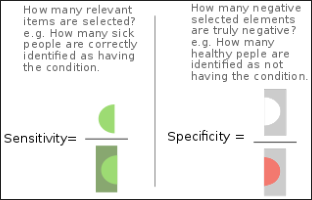
\includegraphics[width=.4\textwidth]{assets/sens-spec-form.png}
\end{cimage}
Si può dire sia che $Sensitivity \equiv Recall \equiv TPR$, sia $Specificity \equiv TNR$.
Mentre la Specificity indica quanto è accurato il sistema: corrisponde alla Recall della \textbf{classe negativa}.
\begin{quote}
    Entrambe le misurazioni sono disponibili sulla diagonale della matrice di confusione normalizzata.
\end{quote}
% subsection Sensitivity e Specificity (end)
%
% section Metriche per la misura di prestazioni (end)
%
\section{Object Detection: AP e mAP}\label{sub:object_detection_ap_e_map} % (fold)
\begin{definition}{Detection}{}
    Per ogni oggetto presente in un'immagine o frame di un video, determina la probabilità di appartenenza alla classe più probabile e la corrispondente bounding box.
\end{definition}
\begin{cimage}
    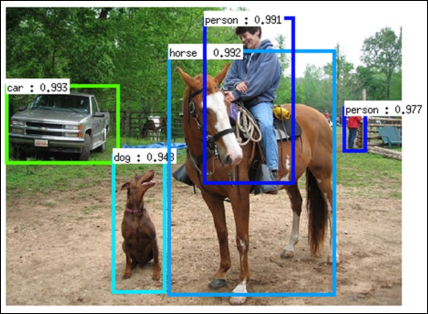
\includegraphics[width=.6\textwidth]{assets/det-sample.png}
    \caption{Esempio di detection di oggetti diversi}\label{fig:det-sample}
\end{cimage}
Diversi sono i tipi di errore, tra cui: oggetto non trovato, classe errata, bounding box sbagliata o imprecisa.
Come si può quantificare il tutto con uno scalare per rendere i sistemi confrontabili?
\\
\begin{itemize}
    \item \textbf{\acf{ap}} è calcolata per oggetti di una singola classe su tutto il database;
    \item \textbf{\acf{map}} è la media di \ac{ap} su tutte le classi;
\end{itemize}
Per calcolare \ac{tp} e \ac{fp} si considera una prediction corretta quando la classe è giusta e la \ac{iou} delle due bounding box (rilevata e vera) è maggiore di un valore scalare dato.
%
\subsection{Problemi Closed e Open set}\label{sec:problemi_closed_e_open_set} % (fold)
Nel caso più semplice, e più comune nei benchmark di machine learning, si assume che il pattern da classificare appartenga a una delle classi note (\textbf{closed set}).
In molti casi reali invece i pattern da classificare possono appartenere a una delle classi note o a nessuna di queste (\textbf{open set}).
\\
Due soluzioni:
\begin{itemize}
    \item si aggiunge alle classi un'ulteriore classe fittizia <<il resto del mondo>> e si aggiungono al training set i cosiddetti <<esempi negativi>>;
    \item si consente al sistema di non assegnare il pattern.
        A tal fine si definisce una \textbf{soglia} e si assegna il pattern alla classe più probabile solo quando la probabilità è superiore alla soglia;
\end{itemize}
\begin{example}{}{}
    Consideriamo un problema id classificazione binario, dove le due classi corrispondono a esempi \textit{Positivi} (vera classe) e \textit{Negativi} (classe fittizia resto del mondo).
    Come in Face detection dove sono positive tutte le porzioni di immagine in cui appaiono i volti, e negative in quelle dove non compaiono.
    \\
    Analogamente possiamo considerare solo la classe \textbf{positivi} e un sistema (con soglia) in grado di calcolare la probabilità $p$ di appartenenza di un pattern alla classe.
    Sia $t$ il valore di soglia, allora il pattern vioene classificato come positivo se $p > t$, come negativo in caso contrario.
\end{example}
% subsection Problemi Closed e Open set (end)
%
\paragraph{Sistemi Biometrici}\label{par:sistemi_biometrici} % (fold)
Un sistema biometrico esegue la \textbf{verifica d'identità} ($1:1$) o \textbf{identificazione} ($1:N$) di un soggetto sulla base di una sua caratteristica fisica o comportamentale.
La verifica d'identità può essere assimilata a un problema di classificazione binario:
\begin{itemize}
    \item False Positive e False Negative in questo caso prendono il nome di \textbf{False Acceptance} e \textbf{False Rejection};
    \item \ac{fpr} e \ac{fnr} prendono il nome di \textbf{\ac{far}} e \textbf{\ac{frr}}.
\end{itemize}
L'identificazione è un problema open set multi'classe.
\begin{quote}
    Gli errori sono \textbf{\ac{fpir}} e \textbf{\ac{fnir}}
\end{quote}
% paragraph Sistemi Biometrici (end)
% section Object Detection: AP e mAP (end)
%
\section{Convergenza}\label{sub:convergenza} % (fold)
Il primo obiettivo da perseguire durante l'addestramento è la \textbf{convergenza} sul Train set.
\\
Consideriamo un classificatore il cui addestramento prevede un processo \textit{iterativo}.
\begin{cimage}
    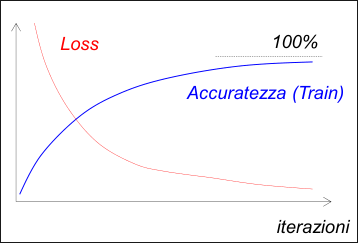
\includegraphics[width=.4\textwidth]{assets/conv.png}
    \caption{Esempio di convergenza}\label{fig:conv}
\end{cimage}
Si ha convergenza quando:
\begin{itemize}
    \item la \textbf{loss} (output della loss function) ha andamento \textbf{decrescente};
    \item l'accuratezza ha andamento \textbf{crescente};
\end{itemize}
\begin{critical}
    \begin{itemize}
        \item se la \textbf{loss} non decresce (o oscilla significativamente) il sistema non converge: 
            \begin{itemize}
                \item il metodo di ottimizzazione non è efficace;
                \item gli iperparamentri sono fuori range;
                \item il learning rate è inadeguato;
                \item ci sono errori di implementazione;
            \end{itemize}
        \item se la loss decresce ma l'accuratezza non cresce, probabilmente è stata scelta una loss-function errata;
        \item se l'accuratezza non si avvicina al $100\%$ sul Train, i gradi di libertà del classificatore non sono sufficienti per gestire la complessità del problema;
    \end{itemize}
\end{critical}
%
\subsection{Generalizzazione e Overfitting}\label{sec:generalizzazione_e_overfitting} % (fold)
Ricordando che l'obiettivo è massimizzare l'accuratezza sul Test.
Nell'ipotesi che Valid sia rappresentativo di Test, si pone l'obiettivo di massimizzare l'accuratezza su Valid.
\\
Per \textbf{generalizzazione} si intente la capacità di trasferire l'elevata accuratezza raggiunta su Train a Valid.
Se i gradi di libertà del classificatore sono eccessivi, si raggiunge elevata accuratezza sul Train, ma non su Valid (scarsa generalizzazione).
In questo caso si parla di \textbf{overfitting} di Train.
Questa situazione si verifica molto facilmente quando Train è di piccole dimensioni.
\begin{cimage}
    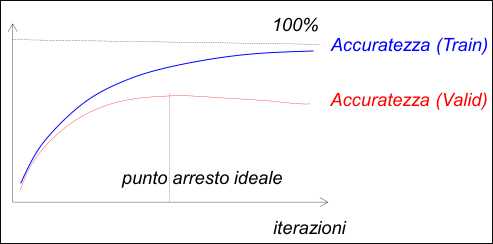
\includegraphics[width=.4\textwidth]{assets/es-overfitting.png}
\end{cimage}
Nei processi di addestramento iterativo, tipicamente dopo un certo numero di iterazioni l'accuratezza su Valid non aumenta più, e può iniziare a decrescere, a causa dell'overfitting.
Monitorando l'andamento si può \textbf{arrestare l'addestramento} nel punto ideale, chiamato \textbf{early stopping}.
\paragraph{Controllare l'Overfitting}\label{par:controllare_l_overfitting} % (fold)
per massimizzare la Generalizzazione.
\\
I gradi di libertà del classificatore non devono essere eccessivi, ma adeguati rispetto alla complessità del problema.
Buona norma partire con pochi gradi di libertà (controllabili attraverso iperparametri) e via via aumentarli monitorando accuratezza su Train e Valid.
\\\\
Inoltre influenzano la regolarità della soluzione appresa, come ad esempio la regolarità del decision boundary nella classificazione o regolarità di una funzione approssimante nella regressione.
La regolarità della soluzione può essere talvolta controllata aggiungendo un fattore regolarizzante alla loss-function che penalizza le soluzioni irregolari.
% paragraph Controllare l'Overfitting (end)
% subsection Generalizzazione e Overfitting (end)
\begin{cimage}
    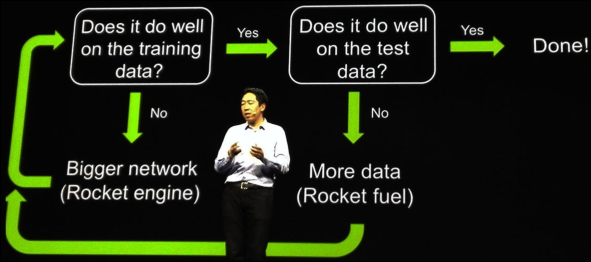
\includegraphics[width=.6\textwidth]{assets/main-recipe.png}
\end{cimage}
% section Convergenza (end)
% chapter Fondamenti (end)
